\part{Minimax search}
\frame{\partpage}

\begin{frame}{Game trees}
	\centering
	\fcolorbox{white}{white}{
		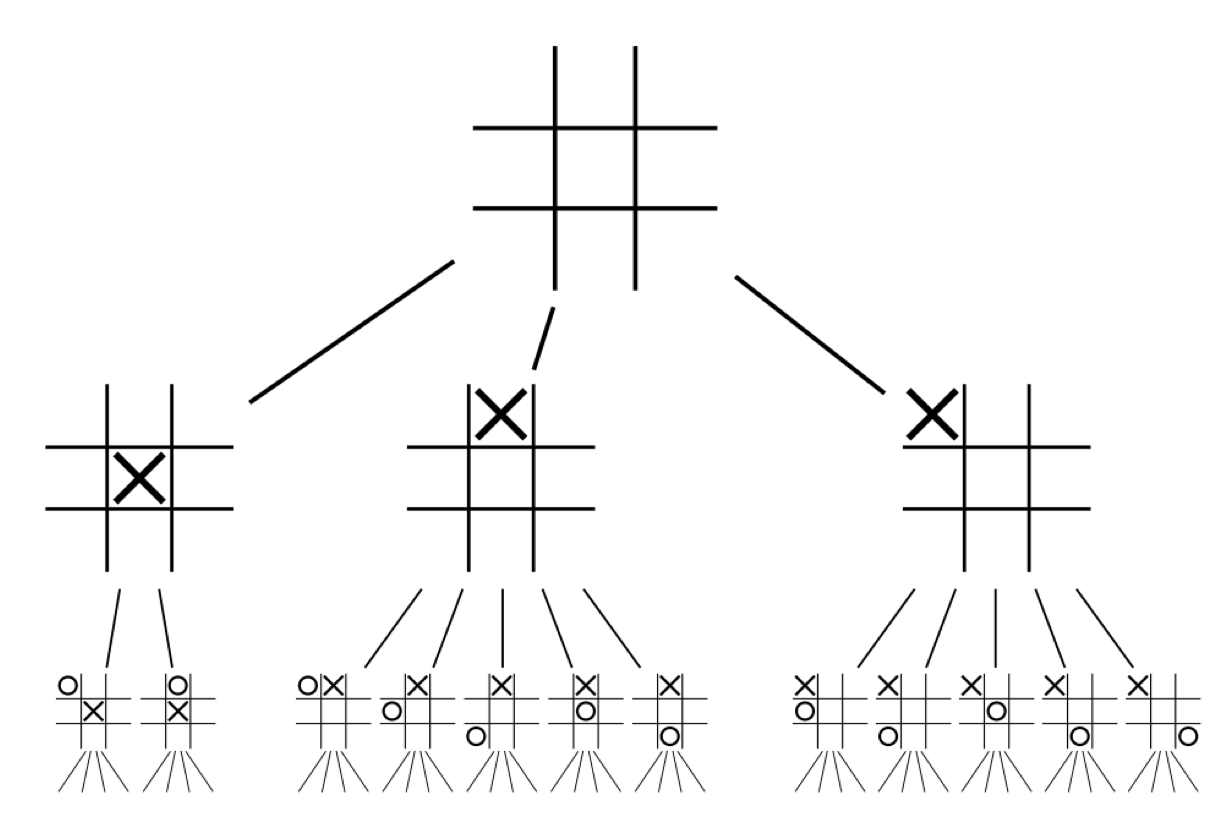
\includegraphics[width=0.8\textwidth]{game_tree}
	}
\end{frame}

\begin{frame}{Minimax}
	\begin{itemize}
		\pause\item Consider a 2-agent MDP with the following restrictions:
			\begin{itemize}
				\pause\item Deterministic
				\pause\item Only one agent chooses an action from a given state
				\pause\item Some states are \textbf{terminal} --- these are the only ones with non-zero reward
				\pause\item The game is \textbf{zero sum}: $R_1(s, a, s') + R_2(s, a, s') = 0$
			\end{itemize}
		\pause\item I want to \textbf{maximise} my reward
		\pause\item My opponent wants to maximise their reward, which is the same as \textbf{minimise} my reward
		\pause\item Therefore I want to \textbf{maximise} the \textbf{minimum} value my opponent can achieve
	\end{itemize}
\end{frame}

\begin{frame}{Minimax search}
	\begin{itemize}
		\pause\item Recursively defines a \textbf{value} for non-terminal game states
		\pause\item Consider each possible ``next state'', i.e.\ each possible move
		\pause\item If it's my turn, the value is the \textbf{maximum} value over next states
		\pause\item If it's my opponent's turn, the value is the \textbf{minimum} value over next states
	\end{itemize}
\end{frame}

\begin{frame}{Minimax search -- example}
\end{frame}

\begin{frame}{Minimax search pseudocode}
	\footnotesize
	\begin{algorithmic}
		\Procedure{Minimax}{state, currentPlayer} \pause
			\If{state is terminal} \pause
				\State \textbf{return} value of state \pause
			\ElsIf{currentPlayer $= 1$} \pause
				\State bestValue $= -\infty$ \pause
				\For{\textbf{each} possible nextState} \pause
					\State $v$ = \Call{Minimax}{nextState, $3 -$ currentPlayer} \pause
					\State bestValue = \Call{Max}{bestValue, $v$} \pause
				\EndFor
				\State \textbf{return} bestValue \pause
			\ElsIf{currentPlayer $= 2$} \pause
				\State bestValue $= +\infty$
				\For{\textbf{each} possible nextState}
					\State $v$ = \Call{Minimax}{nextState, $3 -$ currentPlayer}
					\State bestValue = \Call{Min}{bestValue, $v$}
				\EndFor
				\State \textbf{return} bestValue \pause
			\EndIf
		\EndProcedure
	\end{algorithmic}
\end{frame}

\begin{frame}{Stopping early}
	\begin{algorithmic}
		\For{\textbf{each} possible nextState} 
			\State $v$ = \Call{Minimax}{nextState, $3 -$ currentPlayer}
			\State bestValue = \Call{Max}{bestValue, $v$} 
		\EndFor
	\end{algorithmic}
	\begin{itemize}
		\pause\item State values are always between $-1$ and $+1$
		\pause\item So if we ever have bestValue $= 1$, we can stop early
		\pause\item Similarly when minimising if bestValue $= -1$
		\pause\item There are techniques for smarter early stopping, e.g.\ alpha-beta pruning
	\end{itemize}
\end{frame}

\begin{frame}{Using minimax search}
	\begin{itemize}
		\pause\item To decide what move to play next...
		\pause\item Calculate the minimax value for each move
		\pause\item Choose the move with the maximum score
		\pause\item If there are several with the same score, choose one at random
	\end{itemize}
\end{frame}

\begin{frame}{Minimax and game theory}
	\begin{itemize}
		\pause\item For a \textbf{two-player zero-sum} game
			with \textbf{perfect information} and \textbf{sequential moves}
		\pause\item Minimax search will always find a \textbf{Nash equilibrium}
		\pause\item I.e.\ a minimax player plays \textbf{perfectly}
		\pause\item \textbf{But...}
	\end{itemize}
\end{frame}

\begin{frame}{Minimax for larger games}
	\begin{itemize}
		\pause\item The game tree for noughts and crosses has only a few thousand states
		\pause\item Most games are too large to search fully
			\begin{itemize}
				\pause\item Connect 4 has $\approx 10^{13}$ states
				\pause\item Chess has $\approx 10^{47}$ states
			\end{itemize}
		\pause\item Generally need to \textbf{cut off} the tree at a certain depth and use \textbf{heuristics}
		\pause\item Basically, define our own reward function that (hopefully) approximates the real one
	\end{itemize}
\end{frame}

